\documentclass[11pt,a4paper]{report}

\usepackage[utf8]{inputenc}
\usepackage[T1]{fontenc}

\pagestyle{empty}

\usepackage{graphicx} % Include figure files
\usepackage{amstext,amsbsy,amssymb}
\usepackage{amsmath}
%\usepackage{times} 

%% Numbered problems
\newcounter{excount}[chapter]
\newenvironment{exercise}[1][]{\addtocounter{excount}{1} \noindent {\bf Problem
    \arabic{excount} \ \ #1}\hspace{2mm}}{\vspace{4mm}}


\title{FYS3120 Classical Mechanics and Electrodynamics\\ 
\vspace{15mm}Problem set 5}


%%%%%%%
\begin{document}
%%%%%%%
\maketitle


%%%%%%%%
\begin{exercise}
A particle with mass $m$ moves freely on a horizontal plane. There are no constraints on the motion, but in the following we will consider the free motion described in a rotating reference frame. We refer to the Cartesian coordinates of a fixed frame as $(x,y)$ and the coordinates of the rotating frame as $(\xi,\eta$). They are related by the standard expressions
\begin{eqnarray}
&&x=\xi\cos\omega t-\eta\sin\omega t, \\
&&y=\xi\sin\omega t+\eta\cos\omega t,
\end{eqnarray}
where $\omega$ is the angular velocity of the rotation.

\begin{itemize}
\item[\bf a)] Find the Lagrangian expressed in terms of the coordinates $(\xi,\eta)$ and their time derivatives.
%%%%%%%%%%%%%%%%%%%%%%
\item $\dot{x}=(\dot{\xi} cos \omega t)(-\xi\omega sin \omega t)-(\dot{\eta} sin \omega t)(-\omega \eta cos \omega t)=-\omega \xi \dot{\xi} cos(\omega t)sin(\omega t)+\omega\eta \dot{\eta} cos(\omega t)sin(\omega t)$
\item $\dot{y}=(\dot{\xi}sin\omega t)(\xi\omega cos \omega t)+(\dot{\eta} cos \omega t)(-\omega \eta sin \omega t)=\omega \xi \dot{\xi}sin(\omega t)cos (\omega t)-\omega \eta \dot{\eta} cos( \omega t)sin( \omega t) $

\item \begin{align*}
&v^2=\dot{x}^2+\dot{y}^2  \\
&=\omega^2 \xi^2 \dot{\xi}^2 cos^2(\omega t)sin^2(\omega t)-\omega^2 \xi \eta \dot{\xi} \dot{\eta}cos^2(\omega t) sin^2(\omega t)+\omega^2\eta^2 \dot{\eta}^2 cos^2(\omega t)sin^2(\omega t)\\
&+ \omega^2 \xi^2 \dot{\xi}^2sin^2(\omega t)cos^2 (\omega t)-\omega^2\xi \eta \dot{\xi} \dot{\eta} cos^2(\omega t)sin^2(\omega t)+\omega^2 \eta^2 \dot{\eta}^2 cos^2( \omega t)sin^2( \omega t)\\
&=2\omega^2 \xi^2 \dot{\xi}^2 cos^2(\omega t)sin^2(\omega t)-2\omega^2 \xi \eta \dot{\xi} \dot{\eta}cos^2(\omega t) sin^2(\omega t)+2\omega^2\eta^2 \dot{\eta}^2 cos^2(\omega t)sin^2(\omega t)
\end{align*}
\item $K=\frac{1}{2}mv^2=\frac{1}{2}m(\dot{x}^2+\dot{y}^2)$




\item[\bf b)] Find the corresponding equations of motion for the two variables, and identify the Coriolis and centrifugal terms.
Compare with the standard expression for Newton's second law in a rotating reference frame, as can be found in introductory mechanics text books.
\end{itemize}
\end{exercise}


%%%%%%%%
\begin{exercise}[Midterm Exam 2008]\\
%%%%%%%%%%%
{\em The brachistochrone challenge.}\\
This is a classical problem in analytical mechanics. It was discussed by Galileo Galilei, who suggested a solution (but not the correct one), and studied the problem experimentally. In 1696 the problem was formulated as a challenge to the mathematicians at the time by Johann Bernoulli. He wrote in the journal {\em Acta Eruditorum}:\footnote{Johann Bernoulli, {\em Problema novum ad cujus solutionem Mathematici invitantur,} (A new problem to whose solution mathematicians are invited), Acta Eruditorum 18 (1696) 269.}

\begin{quote}
I, Johann Bernoulli, address the most brilliant mathematicians in the world. Nothing is more
attractive to intelligent people than an honest, challenging problem, whose possible solution
will bestow fame and remain as a lasting monument. Following the example set by Pascal,
Fermat, etc., I hope to gain the gratitude of the whole scientific community by placing
before the finest mathematicians of our time a problem which will test their methods and the
strength of their intellect. If someone communicates to me the solution of the proposed
problem, I shall publicly declare him worthy of praise.
\end{quote}

The problem he formulated was the following:

\begin{quote}
Given two points A and B in a vertical plane, what is the curve traced out by a point acted
on only by gravity, which starts at A and reaches B in the shortest time.
\end{quote}

Five solutions were obtained from scientist and mathematicians we are all acquainted with, Newton,
Jacob Bernoulli (the older brother of Johann), Leibniz and de L'H{\^o}pital, in addition to Johann himself. Johann Bernoulli gave a formulation of the problem where he could use an anology to Snell's law of refraction in optics to solve the problem.

%%%%%%%%%%%%
\begin{figure}[h]
\begin{center}
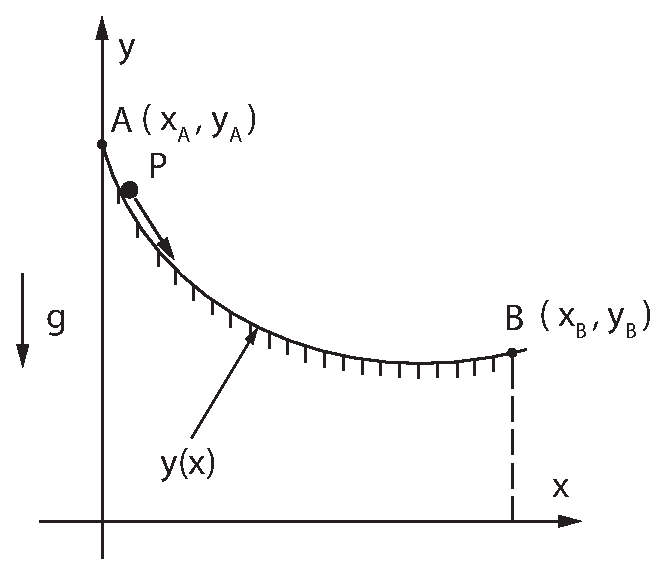
\includegraphics[height=5cm]{Brachistochrone.eps}
\end{center}
\caption{Illustration of the brachistochrone problem.}
\label{fig:brach}
\end{figure}
%%%%%%%%%%%%

Let us now rephrase the problem with a few more words: Assume a small body, named $P$ in Fig.~\ref{fig:brach}, moves in a vertical plane under the influence of gravity only. It leaves a point $A$ with zero velocity and follows (without friction) a given path in the plane which passes through a second point $B$, as shown in the figure. Assume the path between the two points $A$ and $B$ can be changed, while the points themselves stay fixed. For which path between the two points does the body spend the least time on the transit from point $A$ to point $B$? 

The challenge for you is the following: Find the solution to the brachistochrone problem by using the correspondence between the variational problem (finding the ``path of shortest time'') and the Lagrange equation, in the way discussed in the lectures. 

The body $P$ is to be treated as a point particle of mass $m$ and the path is represented by a function $y(x)$ with $x$ as the horizontal and $y$ as the vertical coordinate. The boundary conditions, which fix the positions of point $A$ and $B$, are specified as, $y(x_A)=y_A\,,\;y(x_B)=y_B$. 
To simplify the equations assume in the following that the initial coordinates are $x_A=y_A=0$.

\begin{itemize}
\item[\bf a)] Show that the time $T$  spent by the body on the way between $A$ and $B$ can be expressed as an integral of the form
\begin{equation}
T[y(x)]=\int_{x_A}^{x_B} L(y,y') dx,
\end{equation}
with $y'=\frac{dy}{dx}$, and with 
\begin{equation}
L(y,y')=\sqrt{\frac{1+y'^2}{-2gy}}.
\end{equation}
For the derivation, make use of energy conservation in the form $\frac{1}{2}m v^2+mgy=0$, with $y<0$.
\item[\bf b)] With $L(y,y')$ interpreted as a Lagrangian ($x$ then plays the role of $t$ in the usual formulation) the canonically conjugate momentum is $p=\frac{\partial L}{\partial y'}$ and the Hamiltonian is $H=py'-L$. Explain why $H$ is a constant of motion and use this fact to show that $y(x)$ satisfies a differential equation of the form
\begin{equation}
(1+y'^2)y=-k^2,
\label{eq:diff}
\end{equation}
with $k$ as a constant.
\item[\bf c)] Equation~(\ref{eq:diff}) has a solution which can be written on {\em parametric form} as
\begin{eqnarray}
&&x=\frac{1}{2} k^2(\theta-\sin\theta) \label{eq:parsol_x},\\
&&y=\frac{1}{2} k^2(\cos\theta-1) \label{eq:parsol_y},
\end{eqnarray}
where $\theta$ has been introduced as a curve parameter. Show that (\ref{eq:parsol_x}) and (\ref{eq:parsol_y}) constitute a solution of the differential equation (\ref{eq:diff}) by changing the variable from $x$ to $\theta$ in (\ref{eq:diff}), and by using the above expression for $y(\theta)$. In what way are the boundary conditions taken care of by this solution?
\item[\bf d)]  The curve $y(x)$ defined by the solution of the brachistochrone problem is a section of a {\em cycloid}, known for example as the curve traced out by a point on the periphery of a rolling wheel. Make a plot which shows the form of the curve. 
\item[\bf e)] Assume that point $B$ lies at the lowest point of the cycloid. Show that in this case the following relation has to be satisfied,  $y_B=-\frac{2}{\pi} \,x_B$. Calculate, for that situation, the time used by the body to reach point $B$ from $A$ and compare with the time used when the body instead follows a straight  line between the two points.
\end{itemize}
\end{exercise}


\end{document}

